\section{线性代数}{

  \subsection{向量相关}{

      \subsubsection{标量}{
          标量(scalar),又称纯量,是只有大小,没有方向,可以用实数表示的一个量.实际上标量就是实数,叫他标量只是为了区别于向量.

          标量可以是负数.
      }%标量结尾

      \subsubsection{向量}{
          向量(euclidean vector,物理,工程等也称作矢量,欧几里得向量)是指一个同事具有大小和方向,而且满足平行四边形法则的几何对象.理论数学中向量的定义为任何在向量空间中的元素.一般的,同时具有大小和方向两个性质的几何对象即可认为是向量.向量常常在符号上加以箭头标识来区别于其他两.与向量相对的概念称为标量(数量),即只有大小,绝大多数情况下没有方向,不满足平行四边形法则的量.

          在线性代数中,向量场采用更为抽象的向量空间(也称为线性空间)来定义.向量是所谓向量空间中的基本构成元素.
      }%向量结尾

      \subsubsection{向量表示法}{
          注 : 本笔记默认向量记作头上带一个箭头的符号.比如向量$\alpha$就记作$\vec{\alpha}$

          \begin{itemize}
              \item {
                    向量的代数表示 :

                    代数表示指在指定了一个坐标系之后,用一个向量在该坐标系下的坐标表示该向量.兼具了符号的抽象性和几何形象性,因此具有最高的实用性,被广泛采用与需要定量分析的情形.对于自由向量,将向量的起点平移到坐标原点后,向量就可以用一个坐标系下的一个点来表示,该点的坐标值即向量的终点坐标.

                    设有一向量$\vec{\alpha}$,有坐标系$S$,在$S$中定义好若干个特殊的基本项链(称为基向量,各个基向量共同组成该坐标系下的基)$\vec{e_1},\vec{e_2},\dots,\vec{e_n}$置换,则向量在各个基向量下的投影值即为对应的分量值,各个分量值组成了该向量在坐标系$S$下可唯一表示的一个有序数组(即坐标),且与向量终点一一对应.

                    在矩阵运算中,向量更多的被写成类似于矩阵的列向量或者行向量.在线性代数中所指的向量默认为列向量.比如一个向量$\vec{\alpha} = (a,b,c)$,可写成 : $$
                        \vec{\alpha} = \begin{bmatrix}
                            \alpha_1 \\
                            \alpha_2 \\
                            \alpha_3 \\
                        \end{bmatrix}
                    $$
                    或者行向量的形式 : $$
                        \vec{\alpha} = \begin{bmatrix}
                            \alpha_1 & \alpha_2 & \alpha_3
                        \end{bmatrix}
                    $$

                    列向量和行向量都可以被视为矩阵.
                    }
              \item {
                    向量的几何表示 :

                    直观上,向量通常被标示为一个带箭头的有向线段.线段的长度表示向量的大小(或称模长),向量的方向即箭头所指的方向,可以记为$\vec{\alpha}$.该种表示的优点是具有强烈的几何直观形象性,缺点是在纸面上作图繁琐,不便定量分析 :

                    \begin{center}
                        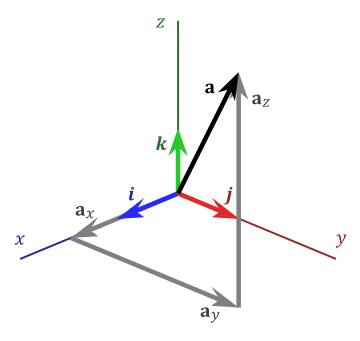
\includegraphics[scale=0.5]{resources/Vector_picture.png}
                    \end{center}
                    }
          \end{itemize}
      }%向量表示法

      \subsubsection{向量空间}{
          \begin{itemize}
              \item 向量空间是现代数学中的一个基本概念.是线性代数研究的基本对象.
              \item 向量空间的一个直观模型是向量几何,几何上的向量及相关的运算即向量加法,标量乘法,以及对运算的一些限制如封闭性,结合律,已大致地描述了"向量空间"这个数学概念的直观形象.
              \item 在现代数学中,"向量"的概念不仅限于此,满足下列公理的任何数学对象都可被当作向量处理.譬如,实系数多项式的集合在定义适当的运算后构成向量空间,在代数上处理是方便的.单变元实函数的集合在定义适当的运算后,也构成向量空间,研究此类函数向量空间的数学分支称为泛函分析.
          \end{itemize}

          给定域$F,F$上的向量空间$\vecSpace$是一个集合,其上定义了两种二元运算:

          \begin{itemize}
              \item 向量加法$+$ : $\vecSpace \times \vecSpace \to \vecSpace$,把$\vecSpace$中的两个元素$\vec{u}$和$\vec{v}$映射到$\vecSpace$中另一个元素,记为$\vec{u} + \vec{v}$
              \item 标量乘法$\cdot$ : $F \times \vecSpace \to \vecSpace$,把$F$中的一个元素$a$和$\vecSpace$中的一个元素$\vec{u}$变为$\vecSpace$中的另一个元素,记作$a \cdot \vec{u}$
          \end{itemize}

          V中的元素称为向量,相对地,F中的元素称为标量.

          而集合V满足以下公理才构成一个向量空间(对F中的任意元素a,b以及V中的任意元素u,v,w都成立):

          \begin{center}
              \begin{tabular}{|l|l|}
                  \hline
                  向量加法的结合律           & $\vec{u} + (\vec{v} + \vec{w}) = (\vec{u} + \vec{v}) + \vec{w}$                                            \\
                  \hline
                  向量加法的交换律           & $\vec{u} + \vec{v} = \vec{v} + \vec{u}$                                                                    \\
                  \hline
                  向量加法的单位元           & 存在一个零向量$\vec{0} \in \vecSpace$,使得对任意$\vec{u} \in \vecSpace$都满足$\vec{u} + \vec{0} = \vec{u}$ \\
                  \hline
                  向量加法的逆元素           & 对任意$\vec{v} \in \vecSpace$都存在其逆元素$-\vec{v}$,使得$\vec{v} + (-\vec{v}) = \vec{0}$                 \\
                  \hline
                  标量乘法与标量的域乘法相容 & $a(\vec{u} + \vec{v}) = a\vec{u} + a\vec{v}$                                                               \\
                  \hline
                  标量乘法的单位元           & 域$F$存在乘法单位元$1$满足$1\vec{v} = \vec{v}$                                                             \\
                  \hline
                  标量乘法对向量加法的分配律 & $a(\vec{u} + \vec{v}) = a\vec{u} + a\vec{v}$                                                               \\
                  \hline
                  标量乘法对域加法的分配律   & $(a + b)\vec{v} = a\vec{v} + b\vec{v}$                                                                     \\
                  \hline
              \end{tabular}

              向量空间的公理定义
          \end{center}

          由这些公理可以推出以下性质 :

          \begin{itemize}
              \item 零向量$\vec{0}$是唯一的.
              \item 对任意$a \in F,a \cdot \vec{0} = \vec{0}$.
              \item 对任意$\vec{u} \in \vecSpace,0 \times \vec{u} = \vec{0}$($0$是$F$的加法单位元).
              \item 如果$a \cdot \vec{u} = \vec{0}$,那么要么$a = 0$,要么$\vec{u} = \vec{0}$.
              \item 向量加法的逆向量$\vec{v}$是唯一的,记作$-\vec{v},\vec{u} + (-\vec{v})$也可以写称$\vec{u} - \vec{v}$,两者都是标准的.
              \item 对任意$\vec{u} \in \vecSpace,-1 \cdot \vec{u} = -\vec{u}$
              \item 对任意$a \in F$以及$\vec{u} \in \vecSpace,(-a) \cdot \vec{u} = -(a \cdot \vec{u}) = a \cdot (-\vec{u})$
          \end{itemize}
      }%向量空间结尾

  }%向量相关结尾

 }%线性代数结尾